\section{Forelesning 13 (Mandag \date{17. februar 2025})}
\paragraph{Hyperbolic conservation laws}
Euler's equations in Gas Dynamics
\begin{align*}
  \rho_t + (\rho u)_x           & = 0 \\
  (\rho u)_t + (\rho u^2 + p)_x & = 0 \\
  E_t + (u(E + p))_x            & = 0
\end{align*}
where \(\rho\) is the density, \(u\) is the velocity, \(p\) is the pressure, and \(E\) is the total energy.

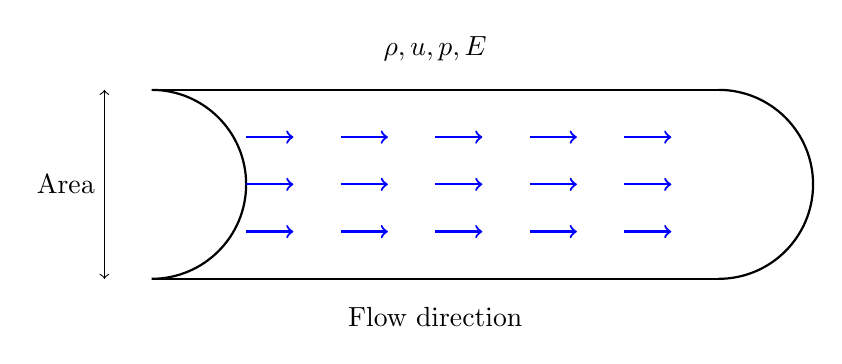
\begin{tikzpicture}[scale=1.2]
  % Draw the tube
  \draw[thick] (0,1) -- (6,1);
  \draw[thick] (0,-1) -- (6,-1);

  % Cross section
  \draw[thick] (0,-1) arc (-90:90:1);
  \draw[thick] (6,-1) arc (-90:90:1);

  % Flow arrows
  \foreach \x in {1,2,3,4,5}
    {
      \draw[->,thick,blue] (\x,-0.5) -- (\x+0.5,-0.5);
      \draw[->,thick,blue] (\x,0) -- (\x+0.5,0);
      \draw[->,thick,blue] (\x,0.5) -- (\x+0.5,0.5);
    }

  % Labels
  \node[above] at (3,1.2) {\(\rho, u, p, E\)};
  \node[below] at (3,-1.2) {Flow direction};

  % Cross section labels
  \draw[<->] (-0.5,-1) -- (-0.5,1) node[midway,left] {Area};
\end{tikzpicture}

\begin{itemize}
  \item \(\rho = \rho(x,t)\) is the density of the gas.
  \item \(u = u(x,t)\) is the velocity of the gas.
  \item \(\rho \cdot u = \rho u(x,t)\) is the mass flux (mass per unit time).
  \item \(m(t) = \int_{a}^{b} \rho(x,t) \, dx\) is the mass of the gas in the interval \([a,b]\).
  \item
        \begin{align*}
          \frac{dm}{dt}                                                                       & = \frac{d}{dt} \int_{a}^{b} \rho(x,t) \, dx                                                                \\
                                                                                              & = \int_{a}^{b} \rho_t(x,t) \, dx                                                                           \\
                                                                                              & = \rho(a,t)u(a,t) - \rho(b,t)u(b,t)                                                                        \\
                                                                                              & = -\int_{a}^{b} (\rho(x,t)u(x,t))_x \, dx                                                                  \\
          0                                                                                   & = \int_{a}^{b} \tfrac{\partial}{\partial t}\rho(x,t) + \tfrac{\partial}{\partial x}(\rho(x,t)u(x,t)) \, dx \\
          \frac{\partial}{\partial t}\rho(x,t) + \frac{\partial}{\partial x}(\rho(x,t)u(x,t)) & = 0 \tag{Conservation of mass}                                                                             \\
          \frac{\partial}{\partial t}(\rho u) + \frac{\partial}{\partial x}(\rho u^2 + p)     & = 0 \tag{Conservation of momentum}                                                                         \\
        \end{align*}
        Where \(p = p(\rho, \rho u, E)\) is the pressure and \(E = E(\rho, \rho u, p)\) is the total energy.
        \[
          \frac{\partial}{\partial t}E + \frac{\partial}{\partial x}(u(E + p)) = 0 \tag{Conservation of energy}
        \]
  \item \textbf{Short form in Vector Notation:}
        \begin{align*}
          \begin{bmatrix}
            \rho   \\
            \rho u \\
            E
          \end{bmatrix}_t + \begin{bmatrix}
                              \rho u       \\
                              \rho u^2 + p \\
                              u(E + p)
                            \end{bmatrix}_x & = 0                                                                \\
          p                                 & = p(\rho, \rho u, E) \quad \text{and} \quad E = E(\rho, \rho u, p)
        \end{align*}
  \item In general a hyperbolic conservation law is of the form:
        \begin{align*}
          \symbf{u}_t + \symbf{f}(\symbf{u})_x & = 0                                                                \\
          \symbf{u}                            & = \begin{bmatrix}
                                                     u_1    \\
                                                     u_2    \\
                                                     \vdots \\
                                                     u_n
                                                   \end{bmatrix} \quad \text{is the vector of conserved quantities} \\
          \symbf{f}(\symbf{u})                 & = \begin{bmatrix}
                                                     f_1(\symbf{u}) \\
                                                     f_2(\symbf{u}) \\
                                                     \vdots         \\
                                                     f_n(\symbf{u})
                                                   \end{bmatrix} \quad \text{is the flux vector}
        \end{align*}
  \item \emph{The Jacobian matrix} of \(\symbf{f}(\symbf{u})\rightarrow \symbf{f}'(\symbf{u})\) has real eigenvalues and is diagonalizable.
  \item From now on, we will assume scalar equation.
        \[
          u_t + (f(u))_x = 0
        \]
  \item \emph{Burger's Equation:}
        \[
          u_t + (\frac{1}{2}u^2)_x = 0
        \]
  \item Let \(m(t)= \int_{a}^{b} u(x,t) \, dx\) be the mass of the gas in the interval \([a,b]\).
  \item \emph{Conservation of mass:}
        \[
          \frac{dm}{dt} = \int_{a}^{b} u_t(x,t) \, dx = f(a,t) - f(b,t) \tag{Boundary condition/flux}
        \]
  \item \emph{Conservative Schemes:} One-step schemes are conservative if they satisfy the conservation law:
        \begin{align*}
          U_m^{n+1} & = U_m^n - p \left[F(U_m^n, U_{m+1}^n) - F(U_{m-1}^n, U_m^n)\right] \\
        \end{align*}
        Where \(F(U_m^n, U_{m+1}^n)\) is the numerical flux.
  \item \emph{Why?} Let
        \[\symbf{U}^n = \begin{bmatrix}
            U_1^n  \\
            U_2^n  \\
            \vdots \\
            U_M^n
          \end{bmatrix}
        \]
        be the vector of conserved quantities at time \(t_n\).

        \begin{figure}[H]
          \centering
          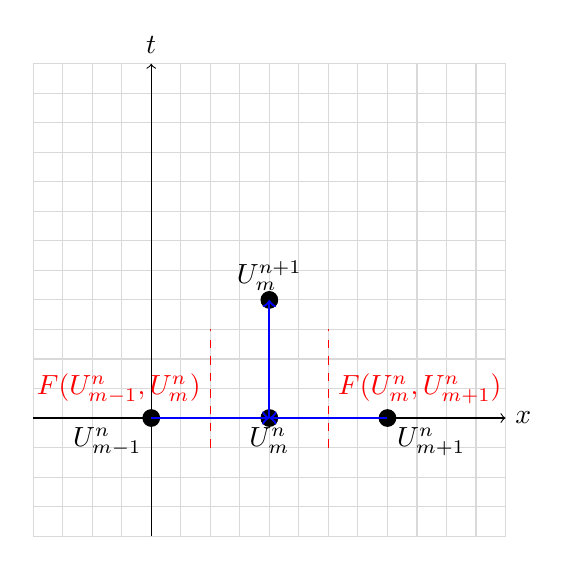
\begin{tikzpicture}[scale=1.5]
            % Grid
            \draw[step=0.25cm,gray!30] (-1,-1) grid (3,3);
            \draw[->] (-1,0) -- (3,0) node[right] {$x$};
            \draw[->] (0,-1) -- (0,3) node[above] {$t$};

            % Points and their labels
            \filldraw[black] (0,0) circle (2pt) node[below left] {$U^n_{m-1}$};
            \filldraw[black] (1,0) circle (2pt) node[below] {$U^n_m$};
            \filldraw[black] (2,0) circle (2pt) node[below right] {$U^n_{m+1}$};
            \filldraw[black] (1,1) circle (2pt) node[above] {$U^{n+1}_m$};

            % Arrows showing dependencies
            \draw[->,thick,blue] (0,0) -- (1,0);
            \draw[->,thick,blue] (1,0) -- (1,1);
            \draw[->,thick,blue] (2,0) -- (1,0);

            % Cell boundaries
            \draw[dashed,red] (0.5,-0.25) -- (0.5,0.75);
            \draw[dashed,red] (1.5,-0.25) -- (1.5,0.75);

            % Flux indicators
            \node[red, left] at (0.5,0.25) {$F(U_{m-1}^n, U_m^n)$};
            \node[red, right] at (1.5,0.25) {$F(U_m^n, U_{m+1}^n)$};
          \end{tikzpicture}
          \caption{Conservative scheme stencil with flux terms}
        \end{figure}
  \item \emph{Trapzoidal Rule for integrating the flux:}
        \begin{align*}
          T(\symbf{U}^n)                                                 & = h \left[ \frac{1}{2}U_0^n + \sum_{m=1}^{M-1} U_m^n + \frac{1}{2} U_M^n \right] \approx \int_a^b u(x,t_n) \, dx  \\
          \frac{d}{dt} m(t_n)                                            & = \frac{1}{k} \left[ m(t_{n+1}) - m(t_n) \right] = \frac{1}{k} \left[ T(\symbf{U}^{n+1}) - T(\symbf{U}^n) \right] \\
          \sum_{m=1}^{M-1} U_m^{n+1}                                     & = \sum_{m=1}^{M-1} U_m^n - p \sum_{m=1}^{M-1} \left[ F(U_m^n, U_{m+1}^n) - F(U_{m-1}^n, U_m^n) \right]            \\
                                                                         & = \sum_{m=1}^{M-1} U_m^n - p \left[F(U_0^n, U_1^n) - F(U_{M-1}^n, U_M^n)\right]                                   \\
          \tfrac{1}{k} \left[T(\symbf{U}^{n+1}) - T(\symbf{U}^n) \right] & = \tfrac{h}{2k} \left[(U_0^{n+1} - U_0^n) + (U_M^{n+1} - U_M^n)\right]                                            \\
                                                                         & \quad + \left[F(U_0^n, U_1^n) - F(U_{M-1}^n, U_M^n)\right]                                                        \\
        \end{align*}
\end{itemize}

\paragraph{Transport Equation}
Let \(p = a \frac{k}{h} \) and \(a > 0\).
\[
  u_t + a u_x = 0
\]
\subparagraph{FTBS Scheme (Upwind)}
\begin{align*}
  U_m^{n+1}                                                                               & = U_m^n - p(U_m^n - U_{m-1}^n)       \\
  \frac{1}{k} \left(U_m^{n+1} - U_m^n\right) + \frac{1}{h} \left(U_m^n - U_{m-1}^n\right) & = 0                                  \\
  U_m^{n+1}                                                                               & = U_m^n - p(f(U_m^n) - f(U_{m-1}^n)) \\
\end{align*}

Conservative with \(F(U_m^n, U_{m+1}^n) = f(U_m^n)\).

Burger's Equation:
\[
  u_t + \frac{1}{2}u^2_x = 0 \quad \text{or} \quad u_t + u \cdot u_x = 0
\]

\subparagraph{Lax-Friedrichs Scheme}
\[
  U_m^{n+1} = \frac{1}{2}(U_{m+1}^n + U_{m-1}^n) - \frac{p}{2}(U_{m+1}^n - U_{m-1}^n)
\]

It is conservative if: \(F(U_m^n, U_{m+1}^n) = \frac{1}{2}(f(U_m^n) + f(U_{m+1}^n))\).

\begin{align*}
  U_m^{n+1} & = U_m^n - \frac{1}{2}\left(U_{m+1}^n - U_m^n + U_{m-1}^n - U_m^n\right) - \frac{p}{2}\left[f(U_{m+1}^n) - f(U_m^n) + f(U_m^n) - f(U_{m-1}^n)\right] \\
            & = U_m^n                                                                                                                                             \\
            & + \frac{1}{2}\left[U_{m+1}^n + U_m^n - p\left(f(U_{m+1}^n) - f(U_m^n)\right)\right]                                                                 \\
            & - \frac{1}{2}\left[U_m^n + U_{m-1}^n - p\left(f(U_m^n) - f(U_{m-1}^n)\right)\right]                                                                 \\
            & = \frac{1}{2}\left[\frac{1}{p} \left(U_{m+1}^n - U_m^n\right) - \left(f(U_{m+1}^n) - f(U_m^n)\right) \right]
\end{align*}

\subparagraph{Lax-Wendroff Scheme}
\[
  U_m^{n+1} = U_m^n - \frac{ap}{2}(U_{m+1}^n - U_{m-1}^n) + \frac{a^2p^2}{2} \partial_x^2 U_m^n
\]

Let \(a(u) = f_u(u)\), then
\[
  u_t + \overbrace{a(u)u_x}^{f(u)} = 0
\]

With the Lax-Wendroff scheme, we get
\begin{align*}
  U_m^{n+1}     & = U_m^n                                                                                     \\
                & - \frac{p}{2}\left[f(U_{m+1}^n) - f(U_{m-1}^n)\right]                                       \\
                & + \frac{p^2}{2}\left[a_{m + 1/2}(U_{m+1}^n - U_m^n) - a_{m - 1/2}(U_m^n - U_{m-1}^n)\right] \\
  a_{m \pm 1/2} & =
  \begin{cases}
    \frac{1}{2}(a(U_m^n) + a(U_{m \pm 1}^n)) & \text{Lax-Friedrichs} \\
    a(\frac{1}{2}(U_m^n + U_{m \pm 1}^n))    & \text{Lax-Wendroff}
  \end{cases}
\end{align*}